\chapter{Metode}
\label{kap:metode}
Vår tilnærming til anvendt rotårsaksanalyse i dette prosjektet er gjennom tre caser som omhandler informasjonssikkerhet. Utførelse av rotårsaksanalyse kan gjøres på ulike måter, men grunnstrukturen er ofte lik. Det handler i bunn og grunn om problemløsning. I tillegg til å analysere casene skal bruken av metoden vurderes ut i fra et kost-nytte perspektiv. Påfølgende seksjon vil forklare valg av metode. 

\section{Metodevalg}
Hovedgrunnen til at rotårsaksanalyse brukes i dette prosjektet er som nevnt tidligere at vi skal undersøke bruksområder for denne analysemetoden i fagfeltet informasjonssikkerhet. Et problem er at rotårsaksanalyse er ikke en standardisert metode. Det er i hovedsak en metode for problemløsning, men det er mange foreslåtte tilnærminger til dette. Et tidligere bachelor-prosjekt \cite{} kom frem til at boka ``Root Cause Analysis: Simplified Tools and Techniques'' av Fagerhaug og Andersen \cite{RCA} beskriver en god og detaljert metode for hvordan rotårsaksanalyse bør utføres. Oppdragsgiver sa seg enig i at dette var et godt utgangspunkt når det skulle jobbes med rotårsaksanalyse, og anbefalte oss metoden. En grunn til at dette er en god metode er den detaljerte oppdelingen av de ulike fasene i RCA. Den skiller seg ut fra de fleste konkurrenter ved å detaljert beskrive hver fase, hvordan du skal gjennomføre den, og ikke minst verktøyene som kan brukes i gjennomføringen. Andre metoder går som regel bare gjennom det generelle hendelsesforløpet og anbefaler et par verktøy som kan brukes. Boken gir en praktisk beskrivelse av hvordan man gjennomfører rotårsaksanalyse. Den beskriver ikke bare hvilke verktøy du burde bruke, men også hvordan du bruker de og i hvilken sammenheng du bør bruke hvert verktøy. Dette bruker boken flytdiagram til å visualisere, og gjør det lett å velge rett verktøy til rett situasjon. Det er spesielt nyttig siden oppgaven vår blant annet dreier seg om å finne ut hvilke verktøy som passer best til informasjonssikkerhetsproblemer. Under er et eksempel på et slikt flytdiagram i første fase av metoden \cite{RCA}.

\begin{figure}[H]
    \centering
    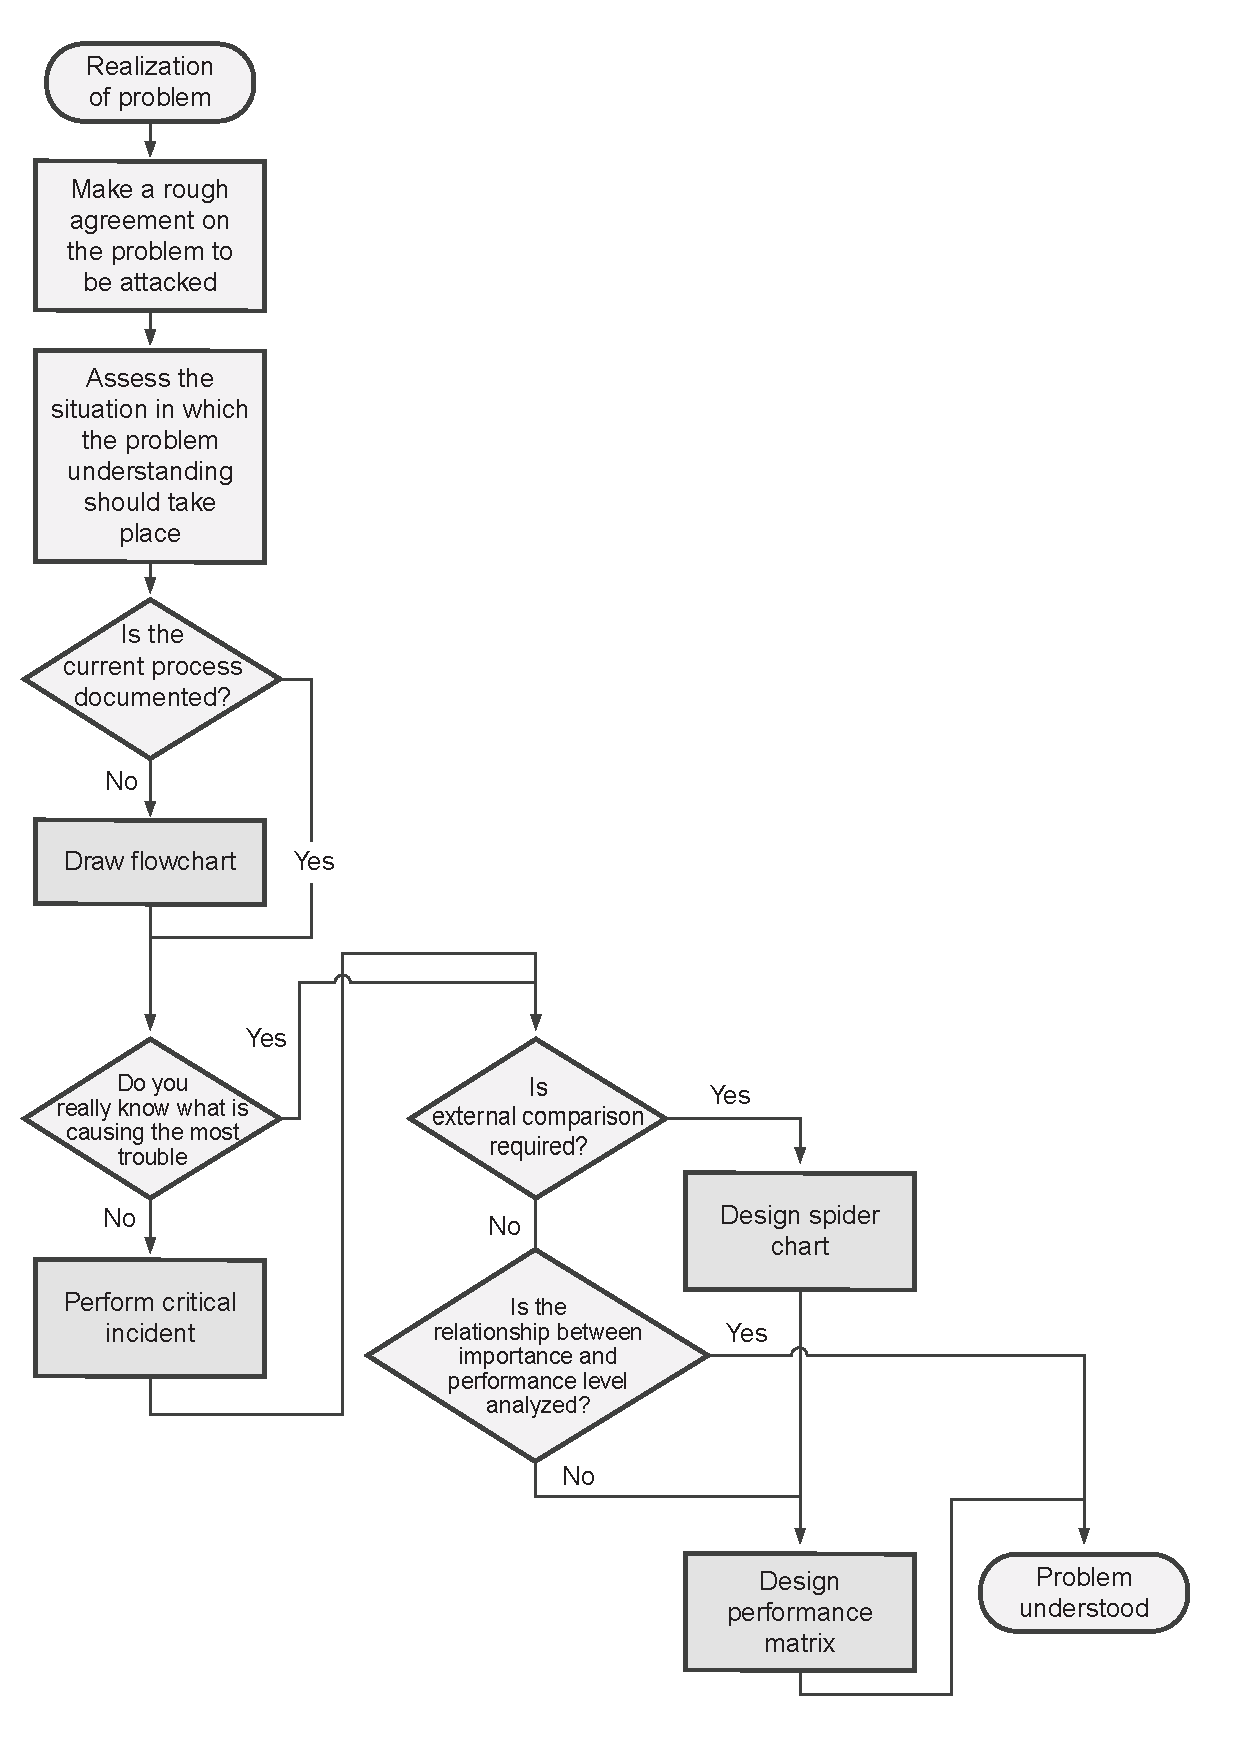
\includegraphics[scale=0.4]{verktoyvalg}
    \caption[RCA-verktoyvalg]{De ulike verktøyene boken anbefaler i første fase ut fra spesifikke kriterier}
    \label{fig:verktoyvalg}
\end{figure}

\section{Metodekritikk}
Selv om metoden er god, har den et par svakheter. For det første er den sekvensiell. Dette gjør at det blir vanskelig å jobbe parallelt og i større grupper. 